% Author: Anwar Baroudi, Rohan Suresh
% Email: mabaroudi@berkeley.edu, rohansuresh@berkeley.edu

\qns{Range Intuition}
\newline
% \begin{figure}[H]
% 	\begin{center}
% 		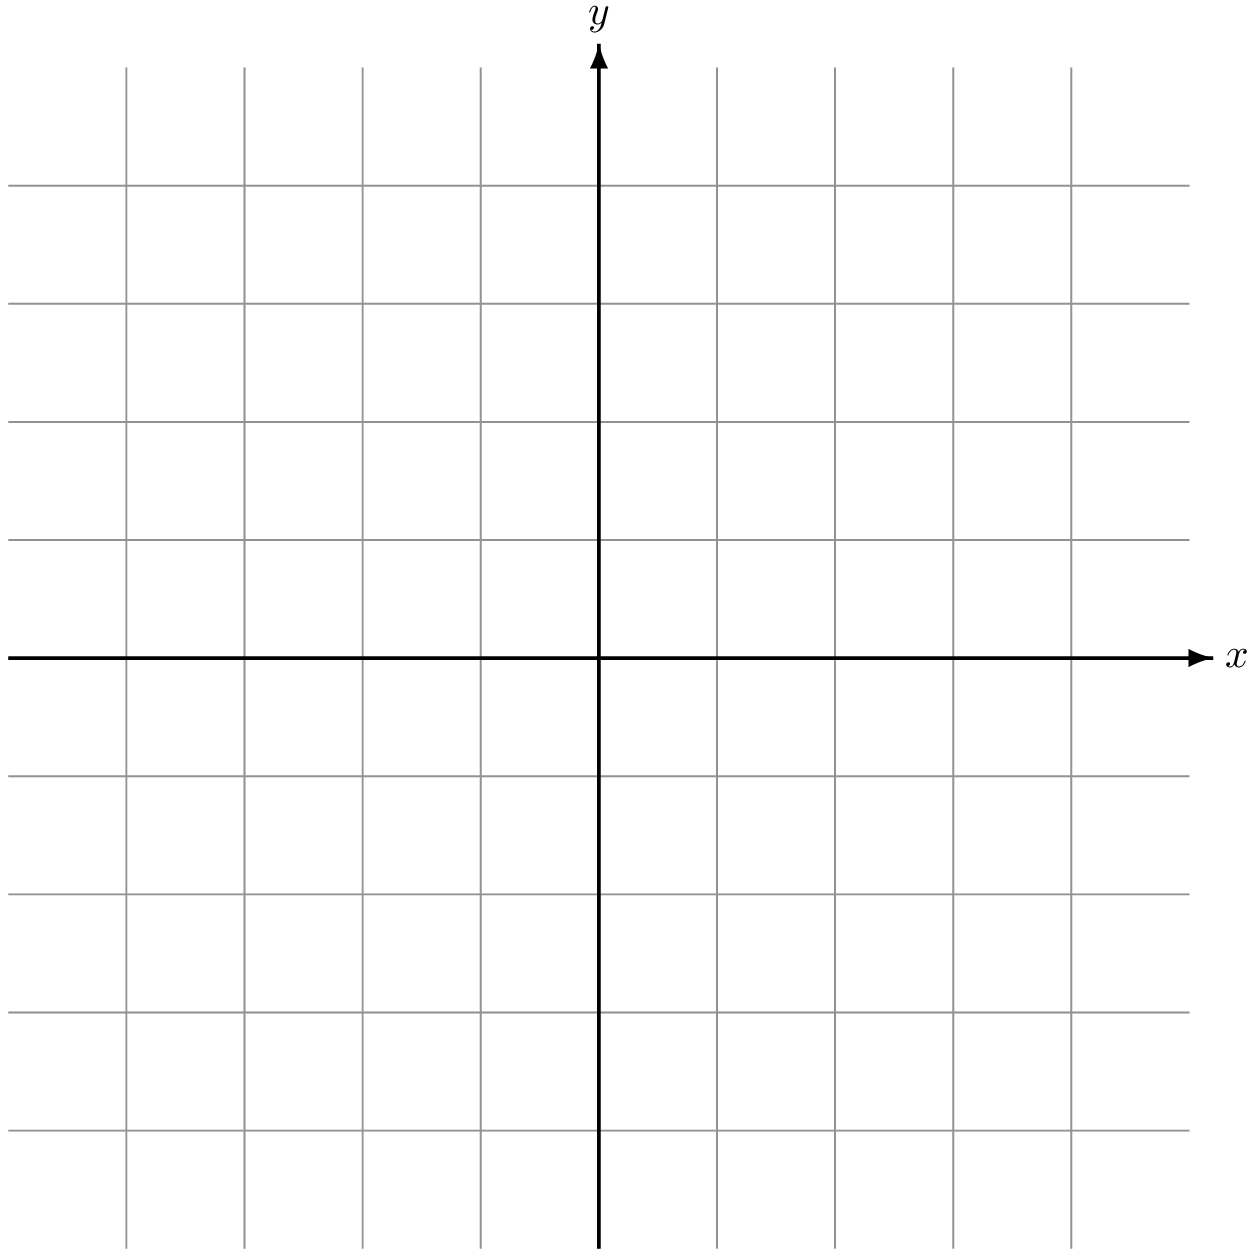
\includegraphics[scale=0.15]{figures/axis.png}
% 	\end{center}
% \end{figure}
\begin{center}
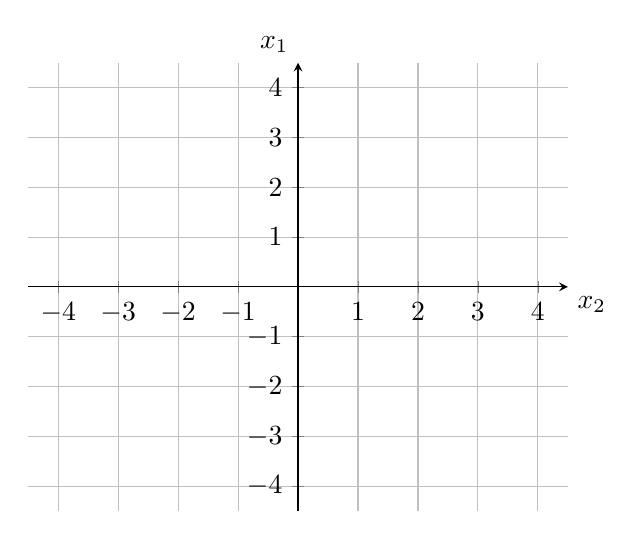
\begin{tikzpicture}[>=latex]
\begin{axis}[
  axis x line=center,
  axis y line=center,
   xtick={-4,...,4},
  ytick={-4,...,4},
  xlabel={$x_2$},
  ylabel={$x_1$},
  xlabel style={below right},
  ylabel style={above left},
  xmin=-4.5,
  xmax=4.5,
  ymin=-4.5,
  ymax=4.5,
  grid]
\end{axis}
\end{tikzpicture}
\end{center}
\[\m{A}=\begin{bmatrix} 1 & 2\\ 1 & 2 \end{bmatrix},\quad \vec{x}=\begin{bmatrix} 3 \\ 1 \end{bmatrix}\]
\begin{enumerate}
\qitem Draw the space on the figure above that is represented by Col($\m{A}$). Also draw the space for the Row($\m{A}$) (which is the same as Col($\m{A}^{\top})$. What dimension are these spaces?

\ans{
The 1 dimensional space for the column space is a line on the $x_2=x_1$ axis (so a diagonal line that goes perfectly northeast, intersecting the origin along the way). The 1 dimensional space for the row space is the line $x_2=2x_1$
}

\sol{
Remember that the lines that are drawn are infinite, make sure to make a point of that.
}

\qitem Plot the point $\vec{x}$, then plot $\m{A}\vec{x}$
% This is how you insert a figure (image figure!)

\ans{
$\mathbf{A}\vec{x}$ should be on the line that represents $\operatorname{Col}(A)$, specifically it should be $\begin{bmatrix}5\\5\end{bmatrix}$
}

\sol{
Make a point of mentioning or having students mention that the result is on the line represented by A, and that this will be true for ALL possible vectors x, to be proved in the next part.
}

\qitem Consider some arbitrary vector $\vec{v}=\begin{bmatrix}v_1\\v_2\end{bmatrix}$ Write out the product $\m{A}\vec{v}$ in terms of $v_1$, $v_2$, and the columns of $\m{A}$.

\ans{
\[
    \m{A}\vec{v} = v_1\begin{bmatrix}1\\1\end{bmatrix} + v_2\begin{bmatrix}2\\2\end{bmatrix}
\]
}

\sol{
    Make sure to make sure students notice the implications of the above answer, that this assures that the result of $Av$ is ALWAYS in the Col($A$). Specifically, make sure they see it written as a sum of scalar-vector products so it's clear that we're only using components in the column space.
}

\qitem We have talked about how matrices like $\m{A}$ have no inverse. Give a geometric explanation for why this is the case. 

\ans{
If we are given some point on the line for the colspace from part (a), we do not know where it came from. For example, if you gave the point given by $\m{A}\vec{x}$, you have no way of knowing that it came from $\vec{x}$
}

\sol{
Make sure students see the ties between independence/invertibility and the geometry.
}

\qitem Consider all points $\vec{y}$ such that $\m{A}\vec{y} = 0$ Draw the space that the $\vec{y}$'s will make up. What do you notice geometrically? What is the dimension of this space?

\ans{
This line should be a straight line that is perpendicular to the line for the row space from part (a). It is a space of dimension 1
}

\sol{
Discuss relationship between colspace and dimension, like how they always add up to the total size of the space.
}
\end{enumerate}
